\documentclass[12pt]{report}
\usepackage{enumitem}
\usepackage[utf8]{inputenc}
\usepackage{graphicx}
\graphicspath{ {images/} }
\usepackage{graphicx}
\begin{document}

\begingroup
\fontsize{18pt}{18pt}\selectfont
\begin{center} 
\centering{  
\textbf{Technische Universit{\"a}t Darmstadt}
 } 
\end{center}
\endgroup

\begingroup
\fontsize{13pt}{13pt}\selectfont
\begin{center} 

  \centering{
Department of Computer Science\\
}
\centering{
Distributed Software System\\
}
\centering{
Telekoperation Lab\\
}
\centering{
 Prof. Dr. Max M{\"u}hlh{\"a}user
}
\end{center}
\endgroup

\newpage
\section*{Acknowledgment}
This Master Thesis was conducted at the Telekoperation Lab (TK) at Technical University Darmstadt in Germany as Masters in Distributed Software Systems (Computer Science).

I would like to thank all the people who contributed in some way to the work described in this thesis.I wish to express my gratitude to Professor Max Müllhäuser for providing me the Possibility to work in a motivating and challenging environment at the TK Lab. I would also like to thank Dipl.-Ing Jens Heuschkel, my advisor and mentor at TK, for encouraging me at every step during my thesis and guiding me through challenging phase of my Thesis. His inputs and suggestions always gave me a future sight to solve the problem. During my tenure, he contributed to a rewarding graduate school experience by giving me intellectual freedom in my work, engaging me in new ideas, and demanding a high quality of work in all my endeavors.

I would also like to thank the researches who were involved in the data validation for this research project. Without the thorough validation of data, the research would not have been successful. I would also like to acknowledge Mr. Anshul Tak of the Ubiquitous Knowledge Processing (UKP) Lab at Technical University Darmstadt as the second reader of this thesis, and I am gratefully indebted to his very valuable comments on this thesis.

Finally, I must express my very profound gratitude to my parents for providing me with unfailing support and continuous encouragement throughout my years of study and through the process of researching and writing this thesis. This accomplishment would not have been possible without them. Thank you.


\newpage

\section*{Introduction and Motivation}
Data mining is the process for extraction of hidden predictive information from large databases, is a powerful new technology with great potential to help companies focus on the most important information in their data warehouses. Researchers in TK Lab have a task of generating pattern or prediction from large amount of Medical data using Machine Learning and data mining. To capitalize the task of Data mining in field of Medical sector, we need bulk amount of data. This data will be provided from CareLink®website. 

Carelink, Web-based system is designed to help take information from all of diabetes management tools –insulin pump, continuous glucose monitor, blood glucose meter(s), and logbook – and organize it into easy-to-read charts, graphs and tables. These reports can help healthcare provider discover trends and other information that can lead to improved therapy management for greater control.
Data crawler is required to access the required data from website without manually visiting it. Web Crawler is the process through which we collect varieties of webpages, in order to gather information from them. Especially with respect to Search Engines, crawlers are used to add index to web pages and it helps in building a database of web sites. It is the system for bulk downloading of web pages. It is a program or automated script, which browses the web in automated manner. Main prominent use of Web crawlers are 

\begin{enumerate}[label=(\alph*)]
\item	Data mining, where web pages are analyzed for statical properties.
\item	Web Search Engines, Indexing web pages.
\item	Web Archiving, where web pages are collected for successors.
\end{enumerate}
There are various types of crawlers available:
\begin{enumerate} [label=(\alph*)]
\item	Incremental crawlers: continuously crawl their crawl space, to get freshness of content.
\item	Batch crawlers: Crawl a snapshot of their crawl space, until reaching a certain sire or time limit.
\item	Focused crawlers: crawl pages to only restricted topics.
\end{enumerate}
Given the overwhelming use of crawler in different scenarios, Web Data mining as a prominent use case for crawling is used in our research project to extract data for Medical research. Jsoup as a Java framework is used to login website https://carelink.minimed.eu/ for bypassing different user agents and manipulating entries in website. Automating downloading CSV file using Web Mining is built with Java Native application.
 (http://webcourse.cs.technion.ac.il/236620/Winter2006-2007/ho/WCFiles/lec14-crawlers.PDF)
Basic Algorithm used for Crawling: 
\begin{enumerate} [label=(\alph*)]
\item	Add the URL in queue.
\item	Until queue is not empty:
\item  Take the first url out of the queue.
\item Retrieve the contents of x from the web
\item Do the needful
\item Mark as visited
\item If x was used as page to find hyperlink URLs
\item Stop when you got the needed Information.
\end{enumerate}

Parallel to accessing data from website, there is also the need of uploading local data to website (server). The process of uploading data to website done using Applet. Since Applet runs only with IE the task of making it automated through browser, simulation has been chosen. Selenium helps automate browsers. It enables java program to emulate user interaction with a web page. Selenium uses Web Drivers for interacting with a Web browser. Web drivers helps to control web browsers by a hook and which in turn enables selenium to interact with web browsers similar to User. Using selenium most of the repeatability of the tests and the speed at which the tests can be executed. There are a number of commercial and open source tools available for assisting with the development of test automation. Selenium is possibly the most widely used open source solution. With the help of selenium, we are trying to automate uploading Data from USB to server and cut the human repeatable work. This will help mass upload data with minimum efforts and time.

We have used Web Technologies and Web crawling added with automation technologies to make the entire process smooth and easy with just one click. JSoup as a Java framework is used to crawl website and visit particular page with ability to manipulate entries. Jsoup is a java HTML parser. It is a java library that is used to parse HTML document. Jsoup provides API to extract and manipulate data from URL or HTML file. It uses DOM, CSS and JQuery-like methods for extracting and manipulating file. This is used to download CSV file with user-entered dates. Jsoup will help in checking login credentials of User and bypass browser agent so that crawling is uninterrupted. After successful login Using Jsoup user input dates will be insert so that required csv file will be downloaded. 


\section*{Background}
In this section, we provide an overview of Web Crawler, Data Crawler, Automation and Data slicing. We start by discussing Web Crawler and Data crawler in Internet and extracting data from webpage. We then move ahead with automating Web browser clicks and manipulation using Selenium as a Internet Explorer WebDriver. At last, we explain the newly built algorithm for Data slicing and recognizing events for it.
\subsection*{Basics of Web Crawling}
Web crawler also called as Web spider or Web Robot is a program, which browses the Web in an automated manner. This entire process is called web crawling or spidering. Web Crawlers are used for automating maintenance task on a Web site, such as validating HTML Codes. A related use is web archiving where in large set of web pages are periodically collected. The most important reason for web crawler lies in the fact that World Wide Web is not a centrally managed repository of information, but millions of independent web content providers. We can also say that web is held together by set of agreed- upon protocol and data formats such as Hypertext Transfer Protocol (HTTP) , the Hypertext Markup Language (HTML) , the Domain Name Service (DNS), the Transmission Control Protocol (TCP) and the robots exclusion protocol. Hence, Web data miners or search engines have few choices as: Adopt a pull model where they will proactively search the web for new or updated information or try to establish a convention and a set of protocols enabling content providers to push content of interest to the aggregators. 

Web servers are highly autonomous that is the barrier of entry to becoming a content provider is quite low, and hence the fact that the web protocols were at least initially extremely simple lowered the barrier even further in fact, this simplicity is viewed by many as the reason why the web succeeded where earlier hypertext systems had failed. Push protocol would have made difficult to set of web protocols and thus raised the barrier of entry for content providers, while the pull model does not require any extra protocols. At the same level, the pull model lowers the barrier of entry for content aggregators as well: Launching a crawler does not require any a priori buy-in from content providers, and indeed there are over 1,500 operating crawlers , extending far beyond the systems employed by the big search engines. Finally, the push model requires a trust relationship between content provider and content aggregator, something that is not given on the web at large — indeed, the relationship between 178 Introduction content providers and search engines is characterized by both mutual dependence and adversarial dynamics. 
Basic Algorithm used for Crawling:
\begin{enumerate} [label=(\alph*)]
\item	Add the URL in queue.
\item	Until queue is not empty:
\item  Take the first url out of the queue.
\item Retrieve the contents of x from the web
\item Do the needful
\item Mark as visited
\item If x was used as page to find hyperlink URLs
\item Stop when you got the needed Information.
\end{enumerate}
Even though the Web crawler algorithm is simple it still has few challenges such as 

\begin{enumerate} [label=(\alph*)]
\item Many of the content provider may try to add misleading information into the body assembled by the crawler.
\item Most of the high throughput crawlers cannot crawl the entire web and they should not as crawling is performed carefully in controlled manner. There must be balance between exploration of important content and exploitation of content already known to be useful.
\item Crawlers should follow “politeness” i.e not impose too much of a burden on the web sites they crawl.
\item Crawlers should achieve high throughput even though many website possess difficult structure for bot.
\end{enumerate}
Sometimes there might be case that crawlers visit sites without approval or they consume resources on system. When crawling websites often issue of “politeness” comes into picture when large amount of pages are accessed. There are also new ways where in websites does not wished to be crawled to make this known to the crawling agent. There are large number of web pages on Internet and it makes the entire process highly complex. However, introduction of various modern Crawlers helps to solve this problem in a more sophisticated way.
\subsection*{Crawler Architecture}

Figure shows high-level architecture of web crawler. It consist of various process running on different machines connected by network. Multiple worker threads are created using crawler and loop work cycles are achieved using worker thread.

	Beginning of every work cycle, URL is fetched from Frontier Data structure,  which distributes URL according to policies mentioned such as politeness. Worker thread invokes the HTTP fetcher. To resolve host component of the URL into the IP address of relevant web server a DNS module is called using fetcher. It tries to connect to the web server, which checks for any robots exclusion rules and attempts to download the web page.
	
 When the download succeeds, the web page can be stored in a repository of harvested web page. Link extractor gets the page, which then parse the page’s HTML content and extracts hyperlinks contained within. Related URLs are passed to URL distributor, which assigns each URL to a crawling process. Most of the hyperlinks refer to pages on same website, assignment to local crawling process is common case. Now the URL is passed through URL fileter and into the duplicate URL eliminator, which in turn maintains set of all URLs.  At last URL priotizer selects a position for the URL in the frontier, based on factors such as estimated page importance or rate of change.
 
 Web Crawler needs to keep track of URL which are already visited and that needs to be visited. There is a flag associated with each URL where page is downloaded or not. Few key functions should be taken into account such as Retrieving a URL, marking a URL as downloaded, adding a new URL and testing whether the set contains a URL. Modern web Crawler are splits into two main data structures as.
 \begin{enumerate} [label=(\alph*)]
\item To maintain the set of URL that have been visited (duplicated URL eliminator”)
\item To maintain set of URL that has to be visited (frontier)
\end{enumerate}

\subsection*{Frontier Data Structure}
First in First out (FIFO) is implemented in Frontier Data structure.  Search will take place as breadth-first traversal of web graph. However, as we know most of the hyperlinks are relative and hence FIFO queue has long runs of URLs on same web server. Is it very common to not issue multiple overlapping request to server. Most of the easy way to realize it is to maintain a mapping between web servers to crawling threads. A separate FIFO queue is assigned to each crawling thread. Another dedicated policy is to send request to each web server depending on server’s capabilities. For instance crawler can delay requests to a server by a multiple of time to get last page from server. Mercator web crawler implements adaptive politeness. Frontier is divided into two parts, “front end” and “back end”.

Front end consisted of a single queue Q, and URLs were added to the frontier byen queuing them into that queue.  Many separate queues are contained in back end. Queue containing URL belongs to a single web server; mapping from web servers to back-end queues are maintained on table T. In addition, associated with each back-end queue q was a time t at which the next URL from q may be processed. These (q,t) pairs were organized into an in-memory priority queue, with the pair with lowest t having the highest priority.  Removing highest-priority entry (q,t) obtained URL by crawling thread from priority queue, waiting if necessary until time t had been reached, dequeuing the next URL u from q, downloading it, and finally reinserting the pair (q,tnow + k · x) into the priority queue, where now is the current time, x is the amount of time it took to download u, and k is a “politeness parameter”; typically 10. If dequeuing u from q left q empty, the crawling thread would remove the mapping from host(u) to q from T, repeatedly dequeue a URL u from Q and enqueue u into the back-end queue identified by T(host(u )), until it found a u such that host(u ) was not contained in T. At this point, it would enqueue u in q and update T to map host(u ) to q.

\subsection*{URL Seen Test (duplicated URL eliminator)}
UrL Seen Test is used to exempt adding multiple instances of the Same URL to the frontier and that is why it is called duplicate URL eliminator. During batch crawling setting UST supports insertion and set membership testing. There are various implementation of UST such as Bloom filter or a hash table. In memory implementation has issues with scaling to large web corpora but they scale well in frontier. Commercial search engines employ distributed crawlers and a hash table realizing the UST can be partitioned across the machines in the crawling cluster.

In the Mercator scheme, adding bunch of URL into disk-based hash file involves reading the old hash file and writing out an updated version. Therefore, the require  time is directly equivalent to the number of discovered URLs. A slight improvement of this pattern is to store the URL hashes on disk in sorted order as before, but lightly packed rather than densely packed. The k highest-order bits of a hash determine the disk block where this hash resides (if it is present). Merging a batch into the disk file is done in place, by reading a block for which there are hashes in the batch, checking which hashes are not present in that block, and writing the updated block back to disk. Thus, the time requirement for merging a batch is proportional to the size of the batch, not the number of discovered URLs (albeit with high constant due to disk seeks resulting from skipping disk blocks). Once any block in the file fills up completely, the disk file is rewritten to be twice as large, and each block contains hashes that now share their k + 1 highest-order bits.

\subsection*{Auxiliary Data Structures}
Web crawlers should adhere to the Robots Exclusion protocol, a convention that allows a web site admins to bar crawlers from crawling.  It is done by providing a file at URL /robots.txt containing rules such as which pages the crawler is allowed to download. Before crawling web site crawler must check if the site supplies /robots.txt file and if it does, crawler should adhere to rules. Some URLs contain a host component (e.g., www.yahoo.com), which is “resolved” using the Domain Name Service (DNS). DNS requests can take quite a long time due to the request forwarding nature of the protocol. Therefore, crawlers often maintain their own DNS caches. As with the robots exclusion rule cache, entries are expired according to both a standard eviction policy, and to expiration directives.

 
\subsection*{Distributed crawling}

To increase the throughput of crawling, web crawler can be distributed over multiple machines. Distributed crawling is achieved by portioning the URL space i.e. node is responsible for a subset of the URLs on the web. URL space is best partitioned across web site boundaries. Politeness policies are best achieved using partitioning the URL across site boundaries. In addition, most of the major data structures can easily be partitioned across site boundaries, i.e., the frontier, the DUE, and the DNS and robots exclusion caches of each node contain URL, robots exclusion rules, and name-to-address mappings associated with the sites assigned to that node, and nothing else.

\subsection*{Incremental crawling}

Snapshots of batch crawling can be assembled using Web crawlers. To perform incremental or continuous crawling where the resources of the crawler are divided between downloading newly discovered pages. For making good Incremental crawling requires few changes to the major data structures of crawlers. DUE should support deletion of URLs that are no longer valid. If URL are priotrized in frontier, the priority of a previously downloaded URL should be dependent on a model of the page’s temporal behavior based on past observations. Other factors such as page quality are also taken into account.

\section*{Selenium}
There are numerous browser automation tools available but the one, which outperforms others and could be found open source is Selenium. Selenium is a browser automation tool; mostly it is used to simulate user interaction on web applications. The browser control is automated so that repetitive tasks can be automated. Looking at the overview of Selenium, it is a combination of selenium IDE, selenium Web driver and selenium gird. Selenium grid helps to use the selenium APIs to control browser instances distributed over a grid of machines. Selenium IDE is an extension for Firefox used to record and playback tests. Selenium uses lot of Jargon.

\begin{enumerate} [label=(\alph*)]
\item Selenium core uses lot of JavaScript that control the browser.
\item Selenium WebDriver binds both language binding and individual browser controlling core.
\item Selenium RC is used for language binding.
\end{enumerate}

Advantages of Selenium:
\begin{enumerate} [label=(\alph*)]
\item Opensource tool
\item No licensing cost
\item Customize according to our requirement
\end{enumerate}

Disadvantage of selenium:
\begin{enumerate} [label=(\alph*)]
\item	There can be cases when selenium fails to recognize objects
\item Online support for selenium is very less
\end{enumerate}

Variant of selenium:
\begin{enumerate} [label=(\alph*)]
\item Selenium IDE
\item Selenium Core
\item Selenium Remote Control
\item Selenium Grid
\end{enumerate}

\section*{WebDriver Design}
WebDriver’s API is also called as  “object-based”. The interfaces are clearly defined and try to manage singe responsibility and hence rather than modelling every single possible HTML Tag we have only one WebElement interface.

\begin{verbatim}
WebDriver driver = new FirefoxDriver();
driver.<user hits space>
driver.findElement(<user hits space>)
driver.findElement(By.id("some_id"));
\end{verbatim}

\section*{IEDriver}
IE browser is constructed of a number of COM interfaces working in concert. Javascript window is an IHTMLWindow.document is an instance of the COM interface  IHTMLDocument. Good thing about IE is that if COM classes works with IE6 it will still continue to work with IE9.

One of the major forces of IE design is that it does not need to have installer. So if there are no installer, there are consequences to this choice. IDE drivers built for selenium are tightly integrated with C\# . Even though c\# would be an attractive language to do the bulk of the coding in, it is not an good option. Something native for the communication to IE and hence C++ as we don’t need to use primary Interloop Assemblies (PIAs). Since we would need to run an installer in order to make that DLL available, we would link our library for communication with IE.

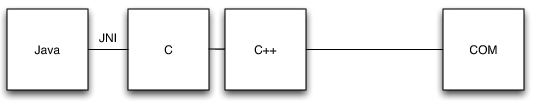
\includegraphics[scale=1]{IEDriver}

Looking at the diagram IE’ COM Automation interfaces are being used and hence to make it easier to manage raw interfaces are wrapped with set of C++ classes that closely mirrored WebDriver API. For Java classes to communicate with C++ JNI is being used. This approach works well with java being only client language but could be very difficult if every other language would require to change the underlying library. So this was not the correct way for abstraction. Every other language had a mechanism of calling down straight C code. In c\# it is PInvoke, In ruby it is FFI, python has ctypes and Java it is JNA(Java Native Architecture. API has to be exposed to lowest common denominator and it was done by taking object model and flattening it, using a simple two or three letter prefix to indicate the "home interface" of the method: "wd" for "WebDriver" and "wde" for WebDriver Element.

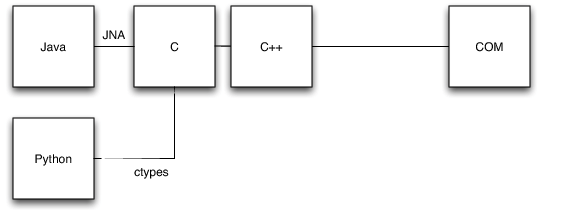
\includegraphics[scale=1]{IEDrivermodified}

On the Java side, we exposed this library of functions via an interface, which we then adapted to make it look like the normal object-oriented interface presented by WebDriver. For example, the Java definition of the \textit{getAttribute} method looks like:
\begin{verbatim}
public String getAttribute(String name) {
PointerByReference wrapper = new PointerByReference();
int result = lib.wdeGetAttribute(parent.getDriverPointer(), element,
 new WString(name), wrapper);
errors.verifyErrorCode(result, "get attribute of");
return wrapper.getValue() == null ? null : new
StringWrapper(lib, wrapper).toString();
}
\end{verbatim}
More and More of IE driver is being moved to sit upon the same Automation qw Firefox. To achieve it we compile each of the atoms as c++ header file, exposing each function as constant. At last, we only have Interaction of API’s in native code and rely on the atoms as much as possible.

\subsection*{Dealing with the combinatorial Explosion}
There is always challenge to minimize cost of maintenance with X browsers supporting Y languages , it would be trap of maintaining X*Y implementations. There can be a way to reduce the number of language that web driver support. It’s always better to write automation scripts in the same language that they work on. There is also a way of reducing the supported browser but it will also not be a feasible solution

\section*{The Remote Driver}
Remote driver is the one of the mechanism to reduce the cost of maintaining web Driver by providing a uniform interface that language binding can code against. Remote driver is used where need to communicate with browser instance that’s running out of process. RPC mechanism is divided into two: transport and encoding. First iteration of the design was developed as a part of Firefox driver. 

Mozilla, and therefore Firefox, was always seen as being a multi-platform application by its developers. In order to facilitate the development, Mozilla created a framework inspired by Microsoft's COM that allowed components to be built and bolted together called XPCOM (cross-platform COM). An XPCOM interface is declared using IDL, and there are language bindings for C and Javascript as well as other languages. Because XPCOM is used to construct Firefox, and because XPCOM has Javascript bindings, it's possible to make use of XPCOM objects in Firefox extensions.

Although futzing with custom encoding protocols over raw sockets is a fun way to pass the time, it has several drawbacks. There were no widely available libraries for the custom protocol, so it needed to be implemented from the ground up for every language that we wanted to support. This requirement to implement more code would make it less likely that generous Open Source contributors would participate in the development of new language bindings. Also, although a line-oriented protocol was fine when we were only sending text-based data around, it brought problems when we wanted to send images (such as screenshots) around.

It became very obvious, very quickly that this original RPC mechanism wasn't practical. Fortunately, there was a well-known transport that has widespread adoption and support in almost every language that would allow us to do what we wanted: HTTP. Below is the diagram of the firefox Driver Architecture

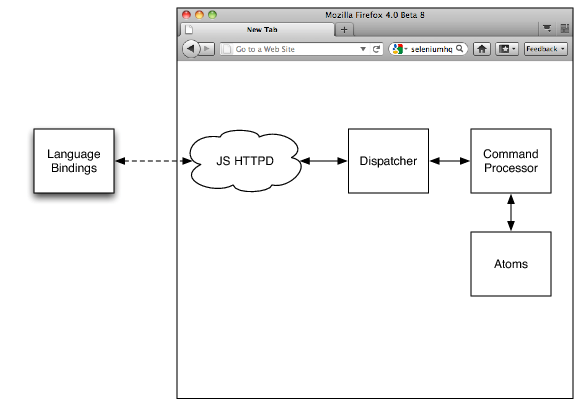
\includegraphics[scale=1]{FireFoxDriver}
The Firefox driver is implemented as a Firefox extension, the basic design of which is shown in Figure 16.4. Somewhat unusually, it has an embedded HTTP server. Although originally we used one that we had built ourselves, writing HTTP servers in XPCOM wasn't one of our core competencies, so when the opportunity arose we replaced it with a basic HTTPD written by Mozilla themselves. Requests are received by the HTTPD and almost straight away passed to a dispatcher object.

The dispatcher takes the request and iterates over a known list of supported URLs, attempting to find one that matches the request. This matching is done with knowledge of the variable interpolation that went on in the client side. Once an exact match is found, including the verb being used, a JSON object, representing the command to execute, is constructed. In our case it looks like:
\begin{verbatim}
{
  'name': 'getElementAttribute',
  'sessionId': { 'value': 'XXX' },
  'parameters': {
    'id': 'some_opaque_key',
    'name': 'rows'
  }
}

\end{verbatim}
This is then passed as a JSON string to a custom XPCOM component we've written called the CommandProcessor. Here's the code:
\begin{verbatim}
var jsonResponseString = JSON.stringify(json);
var callback = function(jsonResponseString) {
  var jsonResponse = JSON.parse(jsonResponseString);

  if (jsonResponse.status != ErrorCode.SUCCESS) {
    response.setStatus(Response.INTERNAL_ERROR);
  }

  response.setContentType('application/json');
  response.setBody(jsonResponseString);
  response.commit();
};
// Dispatch the command.
Components.classes['@googlecode.com/webdriver/command-processor;1'].
    getService(Components.interfaces.nsICommandProcessor).
    execute(jsonString, callback);

\end{verbatim}
There's quite a lot of code here, but there are two key points. First, we converted the object above to a JSON string. Secondly, we pass a callback to the execute method that causes the HTTP response to be sent.
The execute method of the command processor looks up the "name" to determine which function to call, which it then does. The first parameter given to this implementing function is a "respond" object (so called because it was originally just the function used to send the response back to the user), which encapsulates not only the possible values that might be sent, but also has a method that allows the response to be dispatched back to the user and mechanisms to find out information about the DOM. The second parameter is the value of the parameters object seen above (in this case, id and name). The advantage of this scheme is that each function has a uniform interface that mirrors the structure used on the client side. This means that the mental models used for thinking about the code on each side are similar. Here's the underlying implementation of getAttribute
\begin{verbatim}
FirefoxDriver.prototype.getElementAttribute = function(respond, parameters) {
  var element = Utils.getElementAt(parameters.id,
                                  respond.session.getDocument());
  var attributeName = parameters.name;

  respond.value = webdriver.element.getAttribute(element, attributeName);
  respond.send();
};

\end{verbatim}
In order to make element references consistent, the first line simply looks up the element referred to by the opaque ID in a cache. In the Firefox driver, that opaque ID is a UUID and the "cache" is simply a map. The getElementAt method also checks to see if the referred to element is both known and attached to the DOM. If either check fails, the ID is removed from the cache (if necessary) and an exception is thrown and returned to the user.

The second line from the end makes use of the browser automation atoms discussed earlier, this time compiled as a monolithic script and loaded as part of the extension.
In the final line, the send method is called. This does a simple check to ensure that we only send a response once before it calls the callback given to the execute method. The response is sent back to the user in the form of a JSON string, which is decanted into an object that looks like (assuming that getAttribute returned "7", meaning the element wasn't found):
\begin{verbatim}
{
  'value': '7',
  'status': 0,
  'sessionId': 'XXX'
}
\end{verbatim}
This suggests that browsing the web in a copy of Firefox with the WebDriver extension installed is a seriously bad idea as it makes it trivially easy for someone to remotely control the browser.
Behind the scenes, there is a DOM messenger, waiting for the webdriverCommand this reads the serialized JSON object and calls the execute method on the command processor. This time, the callback is one that simply sets the response attribute on the document element and then fires the expected webdriverResponse event.

\end{document}
